\section{Результаты}

В данном разделе будут описаны результаты экспериментов и сравнения разных подходов, так же сделаны некоторые выводы. Все показатели моделей представленных в данной работе отобраны из лучших checkpoint'ов. Стоит отметить, что показатели даны в качестве справки, так как в данном исследовании основной целью было построить рабочий framework и протестировать его на доступном датасете. Так как сам датасет очень шумный из-за разметки с использованием distant supervision, результаты моделей недостаточно высоки.

\subsection{Базовая модель}   В качестве лучшего существующего подхода для извлечения атрибутов из реплик была выбрана модель GKTY представленная в статье \cite{gtky}. Она выбрана в качестве базовой модели, так как из всех существующих похожих подходов она решает поставленную задачу как есть, без дополнительных условностей. Модель состоит из трех компонент:

\begin{itemize}
    \item encoder входной реплики (bidirectional GRU \cite{gru}) для получения эмбеддингов;
    \item классификатор предикатов: multi-hop end-to-end memory network \cite{sukhbaatar2015} которая хорошо показала себя в задаче ответов на вопросы. Решает задачу multi-label classification;
    \item генератор сущностей (GRU \cite{gru}) который по скрытому состоянию encoder'a и предсказанному множеству предикатов генерирует соответствующие субъект и объект.
\end{itemize}

Стоит заметить, что все три компоненты этой архитектуры обучаются вместе в сквозном режиме. В PipelineAE каждая компонента может обучаться параллельно. Также можно заметить, что GenAE тоже напоминает базовую модель, так как одна архитектура решает сразу несколько задач, но все происходит неявно во время оптимизации одной функции потерь \ref{lm_loss}, в то время как у базовой модели используется взвешенная сумма разных функций потерь под каждую задачу.

\subsection{Классификатор предикатов}
В PipelineAE требуется оценить качество каждой компоненты по отдельности. В Таблице \ref{table:rel_cls_results} даны оценки качества классификации предикатов. Предсказания каждого подхода непосредственно или с некоторым преобразованием сводятся к multi-label classification, поэтому даны показатели метрик описанных в разделе экспериментов для multi-label классификации. Для binary ranking и contrastive learning даны результаты после подбора оптимального порога на валидационной выборке. Можно увидеть, что применение multi-label classification без подбора весов для положительных классов сильно смещается в сторону пустого целевого набора предикатов. Об этом говорят нулевая точность (precision) и полнота (recall), то есть модель не дает на выходе 1. Благодаря этому, accuracy этой модели равно доле реплик в датасете в которых нет предикатов вообще. После взвешивания положительных классов, получены результаты чуть лучше, но все равно это очень низко, и модель все еще смещается в сторону 0 в каждом классе. После изучения маргинальных распределений предикатов выяснилось, что и без реплик в которых нет предикатов, в датасете по каждому классу имеется доминирование 0. Тем не менее, после подбора порога получены результаты намного лучше. В случае binary ranking NLI модель показывает самые высокие результаты, уступая по F1 только классификатору предикатов в базовой модели. Тем не менее, более тщательным подбором гиперпамараметров и преобразованием данных можно получить показатели еще выше. Перенос знаних полученных в задаче NLI очевидно в данном случае помогает улучшить результат полученный моделью предобученной на MLM и next sentence prediction. было так же замечено, что из-за своего размера mDeBERTa начала переобучаться и было решено брать checkpoint на ранных стадиях обучения. В случае контрастного обучения, результат представлен у модели, которая обучалась дополнительно с активацией $Sigmoid$ на последнем слое. Хотя, независимо от того, есть сужение значений у функции или нет, модель смещается в сторону предиката "\texttt{<none>}". Чтобы бороться с этим феноменом можно не рассматривать все реплики с нулевым количеством предикатов, так как они очень часто похожи друг на друга, а выбрать среди них случайное подмножество, либо исследовать "сложные" примеры с помощью уверенности модели. Тем не менее, это исследование довольно трудоемко и оставляется на будущее. После подбора порога было замечено, что для достижения оптимального multi-label F1 у моделей в обоих подходах выбирается очень высокий порог. Для binary ranking $\approx 0.87$, а для contrastive learning с активацией $Sigmoid$ $\approx 0.98$. Возможно, это также связано с маргинальными распределениями каждого из предикатов в датасете.

\subsection{Генератор сущностей}
В Таблице \ref{table:egen_results} представлены результаты измерения качества генератора сущностей. Без особых приемов и техник кроме использования описаний предикатов вместо них самих дает достигается высокий результат. Эти показатели можно брать за потолок, который можно достичь с классификатором предикатов.

\begin{table}[!ht]
\centering
\begin{tabular}{c c c}
    & \textbf{F1} & \textbf{ACC} \\
    \hline
    \hline
    mBERT MC weighted & 14.09 & 17.11 \\
    \hline
    mBERT MC weighted (с подбором порога) & 30.03 & 41.4 \\
    \hline
    mBERT MC & 0.0 & 52.04 \\
    \hline
    DistilBERT CL & 28.38 & 26.39 \\
    \hline
    DistilBERT BR & 33.39 & 42.86 \\
    \hline
    mDeBERTa NLI BR & 38.9 & \textbf{45.64} \\
    \hline
    Базовый классификатор предикатов & \textbf{44.40} & 41.57 \\
    \hline
\end{tabular}
\caption{Результаты качества классификации предикатов. BR - binary ranking, CL -contrastive learning, MC - multi-label classification}
\label{table:rel_cls_results}
\end{table}

\begin{table}[!ht]
\centering
\begin{tabular}{c c c c}
    & \textbf{ACC} & \textbf{F1} & \textbf{BLEU-1} \\
    \hline
    \hline
    mT5-small & \textbf{70.3} & \textbf{70.6} & \textbf{96.55} \\
    \hline
    Базовый генератор сущностей & 43.48 & 46.03 & - \\
    \hline
\end{tabular}
\caption{Результаты качества генерации сущностей по заданной реплике и правильному предикату.}
\label{table:egen_results}
\end{table}

\subsection{Итоговые метрики}

В Таблице \ref{table:final_results} даны показатели оценок итоговых моделей. Как можно увидеть, почти все подходы представленные в данной работе оказались лучше чем модель GTKY, что показывает превосходство трансформерной архитектуры в данной задаче. Контрастное обучение не дало удовлетворительного результата, что требует дальнейшего более подробного исследования и анализа. Самый лучший результат у модели с классификатором предикатов NLI binary ranking. Следует заметить, что всех моделях в двух-этапном подходе меняется только классификатор предикатов, а генератор сущностей один и тот же. Важно заметить, что показатели генератора сущностей сильно занижаются из-за качества классификации предикатов.

На Рисунке \ref{fig:preds_distr} изображены распределения количества разных сгенерированных триплетов по репликам у различных подходов. Можно увидеть, что mT5 очень редко генерируют больше одного триплета. Только взяв модель базового размера можно было наблюдать заметный скачок в качестве и в распределении предсказанных триплетов. Так же, было замечено, что часто mT5 генерирует один и тот же триплет дважды либо даже 12 раз. Это, возможно, следствие жадного декодинга который использовался во всех экспериментах с генерацией, либо неконсистентный порядок в наборе целевых триплетов, что мешает авторегресссионной модели усваивать правильную последовательность триплетов если их несколько. Распределение триплетов предсказанных GenAE больше всех похоже на распределение в тестовой выборке на Рисунке \ref{fig:triple_distr}.

\begin{table}[!ht]
\centering
\begin{tabular}{c c c c}
    & \textbf{ACC} & \textbf{F1} & \textbf{BLEU-1} \\
    \hline
    \hline
    PipelineAE с mBERT-base MC weighted & 39.17 & 38.9 & 68.68  \\
    \hline
    PipelineAE с DistilBERT BR & 35.64 & 38.06 & 68.49  \\
    \hline
    PipelineAE с DistilBERT CL & 25.8 & 26.73 & 66.39 \\
    \hline
    PipelineAE с mDeBERTa NLI BR & 40.49 & 43.13 & 70.84 \\
    \hline
    GenAE с mT5-small & 40.25 & 41.28 & 71.92 \\
    \hline
    GenAE с mT5-base & \textbf{45.28} & \textbf{46.11} & \textbf{72.84} \\
    \hline
    Базовая модель & 26.52 & 28.68 & 51.87 \\
    \hline
\end{tabular}
\caption{Итоговые оценки качества моделей для извлечения триплетов из реплик. Показатели получены с подобранным порогом для классификатора предикатов.}
\label{table:final_results}
\end{table}

\begin{figure}[!ht]
    \centering
    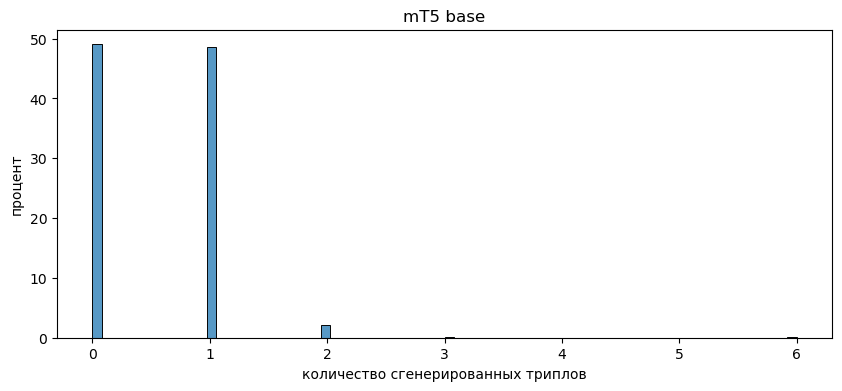
\includegraphics[width=0.9\textwidth]{images/mT5_base_preds_distr.png}
    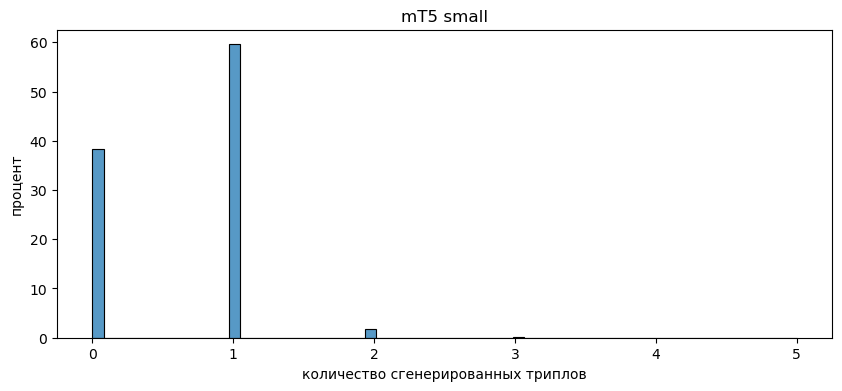
\includegraphics[width=0.9\textwidth]{images/mT5_small_preds_distr.png}
    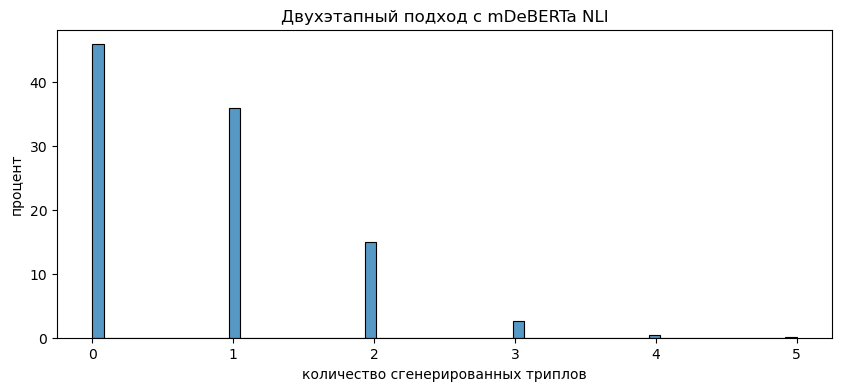
\includegraphics[width=0.9\textwidth]{images/two_stage_preds_distr.png}
    \caption{Распределения количества триплетов в предсказаниях моделей.}
    \label{fig:preds_distr}
\end{figure}
